\section{Git}

\begin{defi}{Git}
    \emph{Git} ist ein verteiltes Open Source-Versionskontrollsystem.
\end{defi}

\begin{defi}{Versionskontrollsystem}
    Durch ein \emph{Versionskontrollsystem} ist es Entwickelnden möglich, Dateien und Verzeichnisse über einen längeren Zeitraum hinweg zu verwalten.
    Dabei ist der Unterschied zum gewöhnlichem Datenspeicher, dass jede Version einer Datei gespeichert wird und man (falls notwendig) auch auf ältere Versionen einer Datei oder eines Projektes zugreifen kann.

    Mit einem Versionsverwaltungssystem kann man sowohl das zeitliche Aufeinanderfolgen von Änderungen als auch das parallele Arbeiten mehrerer Entwickler koordinieren.
    Versionsverwaltung stellt somit ein wichtiges Werkzeug im Softwareentwicklungsprozess dar.

    Viele Versionsverwaltungssysteme sind \emph{zentralisiert}, d.h. es gibt ein zentrales Repository mit allen Dateien und Versionsständen.
    Dabei arbeiten die Entwickelnden normalerweise mit einer lokalen Kopie der aktuellen Version und bringen ihre Änderungen dann in das zentrale Repository ein.

    Im Unterschied dazu ist Git ein \emph{verteiltes Versionsverwaltungssystem}.
    D.h. dass jeder Entwickelnde ein lokales Repository hat und damit arbeiten kann.
    Wenn er eine zusammengehörende Gruppe von Änderungen gemacht und überprüft hat, kann das lokale Repository mit entfernten Repositories synchronisiert werden.

    Durch dieses verteilte Vorgehen von Git sind bestimmte Arbeitsabläufe in der arbeitsteiligen Entwicklung von Software möglich, die in zentralisierten Versionsverwaltungssystemen nur schwer zu erreichen wären.
\end{defi}

\begin{defi}{Arbeitsverzeichnis}
    Das \emph{Arbeitsverzeichnis} enthält den aktuellen Stand des Projektes und alle noch nicht erfassten Änderungen.
\end{defi}

\begin{defi}{Staging Bereich}
    Der \emph{überwachte} bzw. \emph{Staging Bereich} beinhaltet alle Änderungen, die bei einem Commit (Einbringen einer Aktualisierung in das Repository) einer neuen Version dem Repository hinzugefügt werden
\end{defi}

\begin{defi}{Repository}
    Das \emph{Repository} beinhaltet alle Versionen des Projektes.

    Diese werden samt aller Verwaltungsinformationen für das Repository im Ordner \texttt{.git} gespeichert.
\end{defi}

\begin{bonus}{Git Workflow}
    Die Arbeit an einem Projekt erfolgt durch folgende Schritte:
    \begin{enumerate}
        \item Mit \texttt{git clone} wird ein lokales Repository erzeugt, das dann genau der aktuellen Version des entfernten Repostories entspricht.
        \item Nun kann mit diesem Repository lokal gearbeitet werden.
              Alle lokalen Änderungen und Commits sind für andere Entwickelnde desselben Projekts nicht sichtbar.
        \item Möchte man eigene Änderungen für das entfernte Repository zur Verfügung stellen, wird die lokale
              Kopie \enquote{gepusht} und in das entfernte Projekt mittels einem \texttt{git push} eingebracht.
        \item Sollen Änderungen, die andere am entfernten Repository vorgenommen wurden auch lokal verwendet werden, dann holt man sich diese Änderung mit dem Befehl \texttt{git pull}.
    \end{enumerate}
\end{bonus}

\begin{defi}{Tag}
    Manchmal hat man in dem Verlauf einer Projektentwicklung das Bedürfniss eine Version besonders zu kennzeichnen oder hervorzuheben.

    Dies kann durch \emph{Tagging} ermöglicht werden.
    Ein Tag ist einfach eine Markierung, die eine bestimmte Version eines Projektes kennzeichnet.

    Tags werden benutzt, um bestimmte Entwicklungsstände, wie zum Beispiel die Fertigstellung eines Moduls oder eine Auslieferung des Projektes zu einem bestimmten Zeitpunkt zu markieren.
\end{defi}

\begin{bonus}{Git Befehle}
    \begin{center}
        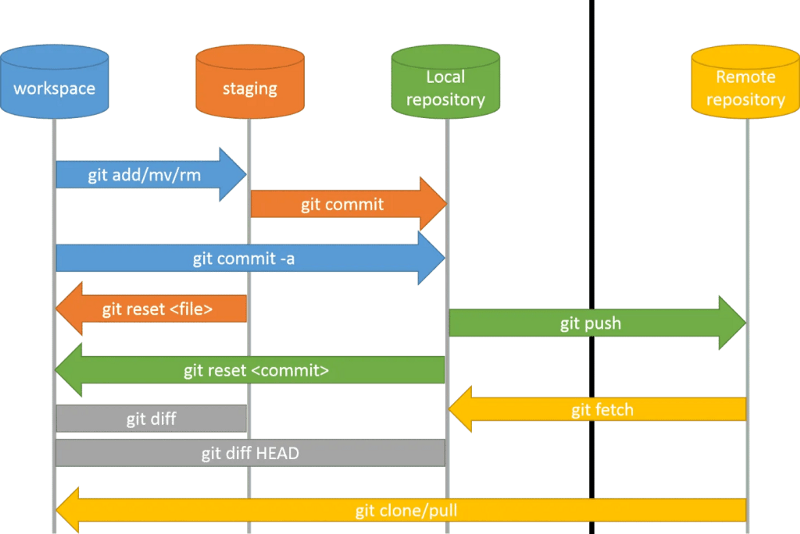
\includegraphics[width=0.9\textwidth]{includes/figures/bonus_git.png}
    \end{center}
\end{bonus}

\begin{defi}{Branch}
    Das Repository wird von Git wie ein Dateisystem mit Historie verwaltet. Jeder Zustand der Dateien in einem Projekt hat einen Versionshash und befindet sich in einer verketteten Liste, die alle Vorgängerversionen in ihrer historischen Reihenfolge enthält.

    An jeder Stelle der Versionskette kann eine Abzweigung, ein \emph{Branch} erzeugt werden.

    Git bietet diverse Möglichkeiten Branches wieder in den Hauptzweig der Entwicklung zu integrieren.
    Im einfachstem Fall entstehen dabei keine Konflikte, weil die Änderungen sich nicht überschneiden.
\end{defi}

\begin{example}{Branch}
    \begin{center}
        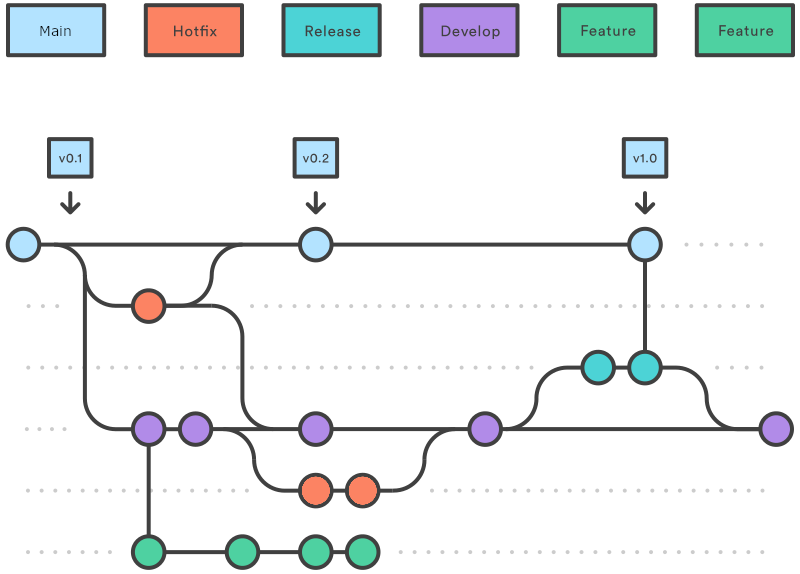
\includegraphics[width=0.9\textwidth]{includes/figures/bonus_git_branches.png}
    \end{center}
\end{example}